\documentclass[12pt]{article}
\usepackage[top=1in, bottom=1in, left=1in, right=1in]{geometry}

\usepackage[onehalfspacing]{setspace}

\usepackage{amsmath, amssymb, amsthm}
\usepackage{enumerate, enumitem}
\usepackage{fancyhdr, graphicx, proof, comment, multicol}
\usepackage[none]{hyphenat}
\usepackage{dirtytalk}
\binoppenalty=\maxdimen
\relpenalty=\maxdimen

\usepackage{microtype}
\usepackage{mathpazo}
\usepackage{mdframed}
\usepackage{parskip}
\linespread{1.1}
\usepackage{graphicx}
\usepackage{subfig}

\usepackage{mathrsfs}
\usepackage{amsfonts}
\usepackage{amsmath}
\usepackage{amssymb}

\usepackage{mathtools}
\newcommand{\defeq}{\vcentcolon=}
\newcommand{\eqdef}{=\vcentcolon}

\newenvironment{statement}[1]
{\begin{mdframed}[linewidth=0.6pt]
        \textsc{Statement #1:}

}
    {\end{mdframed}}

\newcommand{\R}{\mathbf{R}}
\newcommand{\C}{\mathbf{C}}
\newcommand{\Z}{\mathbf{Z}}
\newcommand{\N}{\mathbf{N}}
\newcommand{\Q}{\mathbf{Q}}

\begin{document}
        \noindent
\textbf{Théorie des jeux} \hfill \textbf{Adrien Gourmellet, Lomàn Vezin, Arnaud Corone}\\
\normalsize ECO555 \hfill Date de rendu: 27/11/2020\\

\begin{center}
\textbf{Devoir maison 4}
\end{center}

\textbf{1.} \textit{i.} L'arbre ci dessous représente le jeu décrit sous forme extensive. Les ensembles d'information sont représentés en rouge, ils modélisent le fait que seul le vendeur, $P_{1}$, a connaissance de la qualité de la voiture et que l'acheteur pense que ces deux évènements sont équiprobables. Il semble de plus que selon la donnée $P_{1}$ ne choisit pas la qualité de la voiture qu'il vend. L'aspect aléatoire de la qualité de la voiture qu'il met en vente est donc modélisé par la présence d'un joueur $P_{0}$ qui joue $B$ avec probabilité $\delta$ et $M$ avec probabilité $1-\delta$.
\begin{figure}[htpb]
        \centering
        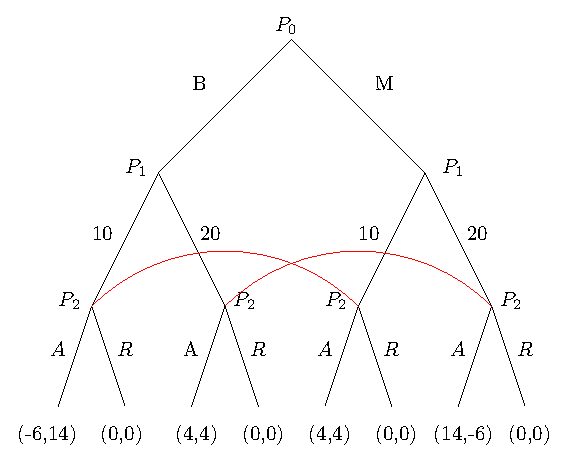
\includegraphics[width=0.8\textwidth]{ext1_2.eps}
        \caption{Forme extensive du jeu}
        \label{fig:ext1}
\end{figure}

\medskip

\textit{ii.} Le joueur 1 dispose de 4 stratégies, \[
(B \to 10, M  \to 10), (B \to 10, M \to 20), (B \to 20, M \to 10), (B \to 20, M \to 20)
.\] On les numérote dans l'ordre de 1 à 4. Le joueur 2 dispose de 2 ensembles d'information avec chacun 2 actions, pour un total de $2\cdot 2 = 4$ stratégies.

Le jeu peut être représenté sous forme normale comme suit
\medskip 

\begin{minipage}{0.4\textwidth}
        \centering
        \begin{tabular}{|c|c|c|c|c|}
                \hline
                & AA & AR & RA & RR \\ 
                \hline
                1 & (-6,14) & (-6,14) & (0,0) & (0,0) \\
                \hline
                2 & (-6,14) & (-6,14) & (0,0) & (0,0) \\
                \hline
                3 & (4,4) & (0,0) & (4,4) & (0,0) \\
                \hline
                4 & (4,4) & (0,0) & (4,4) & (0,0) \\
                \hline
        \end{tabular}
        \captionof{table}{$P_0$ joue $B$}
\end{minipage}
\hfill
\begin{minipage}{0.4\textwidth}
        \centering
        \begin{tabular}{|c|c|c|c|c|}
                \hline
                & AA & AR & RA & RR \\ 
                \hline
                1 & (4,4) & (4,4) & (0,0) & (0,0) \\
                \hline
                2 & (14,-6) & (0,0) & (14,-6) & (0,0) \\
                \hline
                3 & (4,4) & (4,4) & (0,0) & (0,0) \\
                \hline
                4 & (14,-6) & (0,0) & (14,-6) & (0,0) \\
                \hline
        \end{tabular}
        \captionof{table}{$P_0$ joue $M$}
\end{minipage}

Le seul équilibre de Nash est le profil de stratégies \[
        (B \to 20 \; M \to 20, RR)
\] avec paiement $(0,0)$.

\bigskip

\textbf{2.} \textit{i.} L'arbre ci dessous représente le nouveau jeu sous forme extensive. Pour ne pas surcharger l'arbre le joueur 2 joue toujours $A$ à gauche et $R$ à droite.

\begin{figure}[htpb]
        \centering
        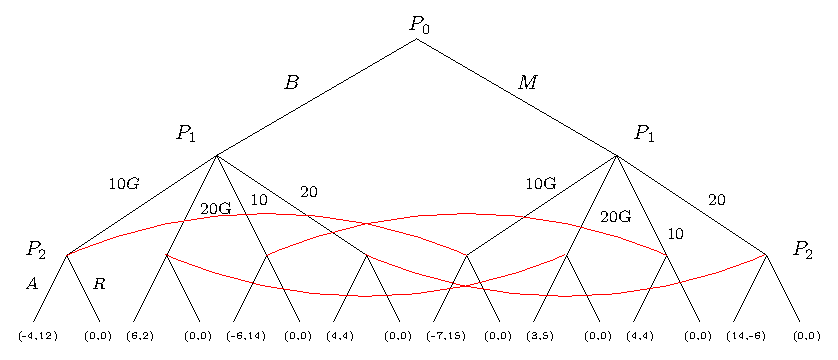
\includegraphics[width=0.8\textwidth]{ext2_2.eps}
        \caption{Forme extensive du nouveau jeu}
        \label{fig:ext2}
\end{figure}

Le joueur 1 a 2 ensembles d'information avec 4 actions chacun pour un total de $4\cdot 4 = 16$ stratégies. De même, le joueur 2 a 4 ensembles d'informations avec 2 actions chacun soit $2^{4} = 16$ stratégies.

La stratégie dans laquelle le joueur 2 n'achète qu'avec garantie \[
        (B \to 20G \; M \to 20G, RRRA)
\] avec paiement $(6,2)$ si la voiture est de bonne qualité et $(3,5)$ si elle est de mauvaise qualité est un équilibre de Nash du jeu modifié.  L'ajout d'une garantie permet de motiver le joueur 2 à ne pas toujours refuser l'échange dans une situation où l'asymétrie de l'information le désavantage.

\end{document}
